\begin{center}
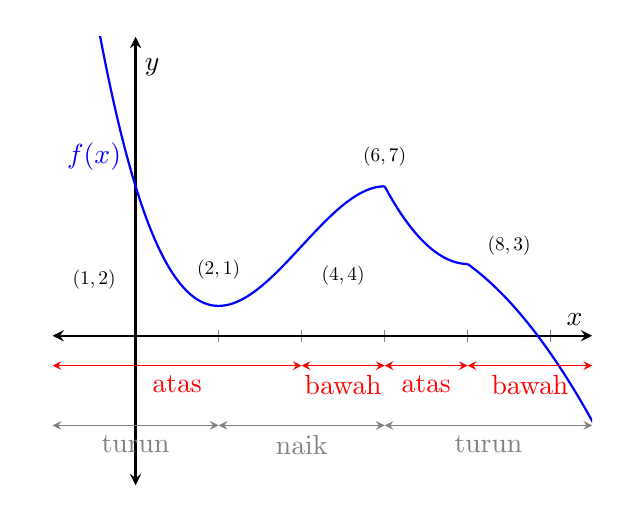
\begin{tikzpicture}[>=stealth]
\begin{axis}[
    xmin=0,xmax=6.5,
    ymin=-5,ymax=10,
    axis x line=middle,
    axis y line=middle,
    y axis line style={draw=none},
    x axis line style={thick},
    y tick style={draw=none},
    axis line style=<->,
    yticklabel=\empty,
    xticklabel=\empty,
    xlabel={$x$},
    ]
    \draw[thick, <->] (1,10) -- (1,-5);

    \addplot[no marks,blue, thick, -] 
        expression[domain=0:4,samples=200]{-(x-2)^3+3*(x-2)^2+1};
    \addplot[no marks,blue, thick, -] 
        expression[domain=4:5,samples=200]{(1.5969*x-8)^2+2.4};
    \addplot[no marks,blue, thick, -] 
        expression[domain=5:8,samples=200]{-(x-4)^2+3.4};

    \point{blue}{(2,1)};
    \node at (2,2.2){\scalebox{0.7}{$(2,1)$}};
    \point{blue}{(1.5,1.875)};
    \node at (0.5,1.875){\scalebox{0.7}{$(1,2)$}};
    \point{blue}{(3,3)};
    \node at (3.5,2){\scalebox{0.7}{$(4,4)$}};
    \point{blue}{(4,5)};
    \node at (4,6){\scalebox{0.7}{$(6,7)$}};
    \point{blue}{(5,2.4)};
    \node at (5.5,3){\scalebox{0.7}{$(8,3)$}};
    \node at (1.2,9){{$y$}};
    \node[blue] at (0.5,6){{$f(x)$}};

    \draw[red, <->] (0,-1) -- node[below](){atas} (3,-1);
    \draw[red, <->] (3,-1) -- node[below](){bawah} (4,-1);
    \draw[red, <->] (4,-1) -- node[below](){atas} (5,-1);
    \draw[red, <->] (5,-1) -- node[below](){bawah} (6.5,-1);
    \draw[gray, <->] (0,-3) -- node[below](){turun} (2,-3);
    \draw[gray, <->] (4,-3) -- node[below](){turun} (6.5,-3);
    \draw[gray, <->] (2,-3) -- node[below](){naik} (4,-3);
\end{axis}
\end{tikzpicture}
\end{center}